\documentclass[conference]{IEEEtran}

\usepackage{url}
\usepackage{multirow}
\usepackage{array}
\usepackage{epsfig}
\usepackage{footnote}
\usepackage{amsmath}
\usepackage{algorithmic}

\setlength{\parskip}{0pt}
\setlength{\parsep}{0pt}
\setlength{\headsep}{0pt}
\setlength{\topskip}{0pt}
\setlength{\topmargin}{0pt}
\setlength{\footskip}{0pt}

\setlength{\topsep}{2pt}
\setlength{\partopsep}{0pt}
\setlength{\itemsep}{0pt}

\setlength{\floatsep}{4pt}
\setlength{\dblfloatsep}{4pt}
\setlength{\textfloatsep}{4pt}
\setlength{\dbltextfloatsep}{4pt}
\setlength{\abovecaptionskip}{4pt}
\setlength{\intextsep}{2pt}

\widowpenalty=10000
\clubpenalty=10000

\begin{document}

\title{On the Design of  Autonomic, Decentralized VPNs}

\author{
\IEEEauthorblockA{
  David Isaac Wolinsky,
  Kyungyong Lee,
  P. Oscar Boykin,
  Renato Figueiredo
}
\IEEEauthorblockN{
  University of Florida
}
}

\maketitle
\begin{abstract}

Decentralized and P2P (peer-to-peer) VPNs (virtual private networks) have
recently become quite popular for connecting users in small to medium
collaborative environments, such as academia, businesses, and homes.  In the
realm of VPNs, there exist centralized, decentralized, and P2P solutions.
Centralized systems require a single entity to provide and manage VPN
server(s); decentralized approaches allow more than one entity to share the
management responsibility for the VPN infrastructure, while existing P2P
approaches rely on a centralized infrastructure but allow users to bypass it to
form direct low-latency, high-throughput links between peers.  In this paper,
we describe a novel VPN architecture that can claim to be both decentralized
and P2P, using methods that lower the entry barrier for VPN deployment compared
to other VPN approaches.  Our solution extends existing work on IP-over-P2P
(IPOP) overlay networks to address challenges of configuration, management,
bootstrapping, and security.  We present the first implementation and analysis
of a P2P system secured by DTLS (datagram transport layer security) along with
decentralized techniques for revoking user access.

\end{abstract}

\section{Introduction}

A Virtual Private Network (VPN) provides the illusion of a local area network
(LAN) spanning a wide area network (WAN) by creating secure\footnote{For the
remainder of this paper, unless explicitly stated otherwise, security implies
encryption and mutual authentication between peers.} communication links
amongst participants.  Common uses of VPNs include secure access to enterprise
network resources from remote/insecure locations, connecting distributed
resources from multiple sites, and establishing virtual LANs for multiplayer
video games and media sharing over the Internet.

The architecture described in this paper addresses usage scenarios where VPNs
are desired but complexity in deployment and management limits their
applicability.  These include collaborative academic environments linking
individuals spanning multiple institutions, where coordinated configuration of
network infrastructure across different sites is often impractical.  Similarly,
small/medium business (SMB) environments often desire the ability to securely
connect desktops and servers across distributed sites without incurring the
complexity or management costs of traditional VPNs.  Such a VPN could be used
to enable extended families to share media among themselves, such as family
videos and pictures, where existing VPNs may be too complicated and where
hosting by centralized service may be undesirable for privacy reasons.

The model of a VPN for collaboration considered in this paper is motivated from
our Archer~\cite{archer} project.  Archer provides a dynamic and decentralized
grid environment for computer architecture researchers to share and access
voluntary compute cycles with each other.  Use of centralized systems would
limit the scope of Archer and require dedicated administration, whereas
existing decentralized solutions require manual configuration of links between
peers, which is beyond the scope of Archer's target users.  Current P2P virtual
network (VN) approaches either lack scalability or proper security components
to be considered VPNs.

We began our original foray into user-friendly VN approaches with
IPOP~\cite{ipop}.  Previous work on IPOP focused on the routing mechanisms and
address allocation with multiple virtual networks (VNs) sharing a single P2P
overlay.  A shared overlay has significant drawbacks as misconfigured or
malicious peers could potentially disable the entire overlay, rendering all VNs
useless.  Though if security and hence isolation is important, prior to VN
deployment, all nodes would need to be configured with a security stack than
the P2P infrastructure prior to deploying the VN system in order to create a
VPN, given the complexity many users would probably reconsider the P2P
approache and use a simple centralized VPN.

To address this challenge, or to make a fully decentralized P2P VPN, in this
paper, we extend the IPOP concept to support bootstrapping from public
infrastructures and overlays into private and secure P2P overlays whose
membership is limited to an individual VPN user base.  Our work is based upon
Castro et al.~\cite{one_ring}, suggesting that a single overlay can be used to
bootstrap service overlays.  We present a practical implementation and
evaluation of this concept.  We then consider security in the overlay and
present the first implementation and evaluation of an overlay with secure
communiation both between end points in the P2P overlay (e.g. VPN nodes) as
well as between nodes connected by overlay edges.  Security requires a means
for peer revocation; however, current revocation techniques rely on centralized
systems such as certificate revocation lists (CRLs). Our proposed approach
allows revocation using scalable techniques provided by the P2P overlay itself.
We call the completed system and the interface used to administrate it {\bf
GroupVPN}, a novel decentralized P2P VPN.

The rest of this paper is organized as follows.  IPOP along P2P overlays are
introduced in Section~\ref{background}.  Throughout the paper, there are two
techniques used to evaluate our approaches, simulation and real system
deployments, these are described in Section~\ref{experimental}.
Section~\ref{private_overlays} describes our techniques that allow users to
create their own private overlays from a shared public overlay in spit of NATs.
Use of security protocols has been assumed in many P2P works though without
consideration of implementation and overheads, we investigate implementation
issues and overheads of security in P2P with emphasis on P2P VPNs in
Section~\ref{security}.  Without revocation, use of security is limited, in
decentralized systems, use of centralized revocation methods do not work, we
present novel mechanisms for decentralized revocation in
Section~\ref{revocation}.  The complete system, GroupVPN, is presented in
Section~\ref{groupvpn}.  Section~\ref{related_work} compares and contrasts our
work with related work.  Section~\ref{conclusions} concludes the paper.

\section{Background}
\label{background}

This section describes the core organization of IPOP, a structured P2P virtual
network, including background on structured overlays, address allocation and
discovery, and connectivity.

\subsection{P2P Overlays}

The type of P2P overlay chosen for a VPN has an effect on how easy the VPN is
to program, deploy, and secure, on its efficiency, and on its scalability.  The
two primary infrastructures for P2P overlays are unstructured and structured
systems.  Unstructured systems use mechanisms such as global knowledge,
broadcasts, or stochastic techniques~\cite{unstruct_v_struct} to search the
overlay. As the system grows, maintaining and searching typically does not
scale.  Alternatively, structured approaches provide guaranteed search times
typically with a lower bound of $O(\log N)$, where N is the size of the
network.  In terms of complexity, for small systems, unstructured systems may
be easier to implement, but as the system grows it may become inefficient.

IPOP uses a structured P2P framework named Brunet~\cite{brunet}, which is based
upon Symphony~\cite{symphony}, a one-dimensional ring with a harmonic
distribution of shortcuts to far nodes.  Structured systems are able to provide
bounds on routing and lookup operations by self-organizing into well-defined
topologies, such as a one-dimensional ring or a hypercube.  Links in the
overlay can be made to guarantee efficient lookup and/or routing times (e.g.
Brunet automatically creates links between peers that communicate often to
achieve efficiency in IP-over-P2P communication).

A key component of most structured overlays is support for decentralized
storage/retrieval of information such as a distributed hash table (DHT).  The
DHT builds upon the existence of a P2P address space.  All peers in a
structured system have a unique, uniformly distributed P2P address.  A DHT maps
look up values or keys (usually by a hashing function) into the P2P address
space.  While there are various forms of fault tolerance, a minimalist DHT
stores values at the node whose address is closest to the value's key.  DHTs
can be used to coordinate organization and discovery of resources, making them
attractive for self-configuration and organization in decentralized
collaborative environments.  As explained in the next section, IPOP, uses a DHT
to coordinate decentralized organization.

\begin{figure*}[ht]
\centering
\includegraphics[width=2.5in,angle=-90]{figs/bootstrap_brunet_light.ps}
\caption{Bootstrapping a private overlay using Brunet}
\label{fig:bootstrap}
\end{figure*}

\subsection{Connecting to the VPN}

To connect to IPOP, a peer needs only to connect to an existing Brunet
infrastructure.  Many IPOP systems can coexist sharing a single overlay.  The
motivation for doing so is that bootstrapping a P2P system can be challenging,
requiring users to have access to public IP addressable nodes or being able to
configure a router or firewall to enable inbound connections.

A peer connected to IPOP's P2P infrastructure can take advantage of its support
for NAT traversal through hole punching~\cite{ice}.  When performing hole
punching, peers first obtain mappings of their private IP address and port to
their public IP address and port and then exchange them over a shared medium,
in this case the P2P overlay.  The peers attempt to simultaneously form
connections with each other, tricking NATs and firewalls into allowing inbound
connections, because the NAT believed an outbound flow already exists, thus
allowing two machines behind two different NATs direct connectivity.  In case
peers cannot establish direct connectivity, messages can be relayed through the
P2P overlay to each other albeit with added latency and reduced throughput.

This approach enables peers behind NATs and firewalls to seamlessly connect to
each other, without requiring peers to host their own bootstrap servers.  The
requirements for a a bootstrap server include a public IP and the ability to
exchange that with users of the system.  Though the system should be redundant
because if a server in a single bootstrap server system goes offline new nodes
will be unable to join the overlay.

\subsection{Network Configuration}

In the context of VPNs, structured overlays can handle organization of the
network space, address allocation and discovery, decentrally through the use of
a DHT. Approaches along these lines have been proposed in~\cite{pcgrid07,i3}.
Membership in the VPN includes a matching membership in the structured overlay,
thus all VPN peers have a P2P address.  To address the challenges of having
multiple VPNs in the same overlay, each IPOP group has its own namespace,
reducing the likelihood of overlap.  To enable scalable and decentralized
address allocation and discovery, peers store mappings of IP address to P2P
address into the DHT, typically of the form $hash(namespace + IP) = P2P
address$.  Thus a peer attempting to allocate an address will insert this (key,
value) pair into the overlay.  The first peer to do this will be the owner of
the IP address allocation.  Therefore the DHT must support atomic writes.

Mechanisms to self-configure the IP address and network parameters of the local
system can be provided by DHCP (decentralized host configuration protocol),
manually configuring the IP address, or the VPN hooking into O/S APIs.  Address
discovery is initiated when an outgoing packet for a remote peer arrives at the
VPN software.  At which point, the VPN will query the DHT with the IP address
to obtain the owner's P2P address and forward the packet to the destination.
Discussion on both these topics is covered in more depth in our previous
work~\cite{sc09}.

\section{Experimental Environment}
\label{experimental}

Throughout this paper, our quantitative evaluation environment uses both real
deployments on PlanetLab and simulation.  The evaluation requirements dictate
the environment used.  When the perspective of a single node is useful,
PlanetLab provides good results, though when attempting to measure detailed
behavior of the entire system using PlanetLab can result in significant noise.

IPOP uses Brunet as the underlying P2P infrastructure for connectivity.  Brunet
has been in active development for the past 5 years and is routinely run on
PlanetLab~\cite{planetlab} for experiments and tests.  PlanetLab consists of of
nearly 1,000 resources distributed across Earth.  In practical applications,
though, roughly 40\% of the resources are unavailable at any given time and the
remaining behave somewhat unpredictably.

PlanetLab deployment takes approximately 15 minutes for all resources to have
Brunet installed and connect to the overlay and then much more time to observe
certain behaviors, making regression and verification tests complicated.  To
address this, we have extended Brunet to support a simulation mode. The
simulator inherits all of the Brunet P2P overlay logic but uses simulated
virtual time based upon an event-driven scheduler instead of real time.
Furthermore, the simulation framework uses a specialized transport layer to
avoid the overhead of using TCP or UDP on the host system, both of which are
limited resources and can hamper the ability to simulate large systems.   The
specialized transport uses datagrams to pass messages between nodes, thus from
the node's perspective, it is very similar to a UDP transport and can simulate
both latency and packet dropping.  Latency between all node pairs is set to 100
ms.

Both simulation and real system evaluation provide unique advantages.
Simulations allow faster than real time execution of reasonable sized networks
(up to a few thousand) using a single resource, while enabling easy debugging.
In contrast, deployment on real systems, in particular PlanetLab, presents
opportunities to add non-deterministic, dynamic behavior into the system which
can be difficult to replicate, such as network glitches and long CPU delays on
processing.

\section{Towards Private Overlays}
\label{private_overlays}

Many users of IPOP begin by using our shared overlay and, once comfortable,
move towards hosting their own infrastructure.  Some are successful without
assistance from us, while a majority are not.  Network configuration issues
tend to be the most common issue preventing users from hosting their own
independent IPOP systems.  While users were able to easily join the shared
overlay, similar attempts to construct their own were hindered and ultimately
only successful after receiving feedback from us.

Bootstrapping a P2P system requires expertise in network administration.  To
enable users to bootstrap their own private overlays, we previously
investigated means by which a public overlay could be used to bootstrap a
private overlay.  Our approach for bootstrapping private systems requires an
overlay to support methods for peers to discover each other, relay messages,
and obtain their public address mapping as described in~\cite{p2p10}.  Examples
of other potential bootstrap overlays include popular and well established P2P
systems, such as Gnutella, Skype, and Kademlia.  Our initial work supports
bootstrapping from XMPP (Jabber) systems and our own P2P overlay, Brunet.  In
this paper, we focus on user perceptions of these technologies with emphasis on
bootstrap times and performance overheads, unlike our previous work, which
verified its utility for bootstrapping private overlays.

To bootstrap from an existing Brunet overlay, peers first insert their public
overlay node address into the key represented by $hash(\$Private Overlay
Namespace)$ and continue to do so regularly until they disconnect, so as to not
let the entry become stale and disappear.  Peers attempting to bootstrap into
the private overlay can then query this key and obtain a list of public overlay
nodes that are currently acting as proxies into the private overlay.  By using
the public overlay as a transport, similar to UDP or TCP, the private overlay
node forms bootstrapping connections via the public overlay.  At which point,
overlay bootstrapping proceeds as normal.  The entire process is represented in
Figure~\ref{fig:bootstrap}.

In a small private overlay, there is a possibility that none of the members
have a public address, making it difficult to provide overlay based NAT
traversal.  Rather than having a special case for NAT traversal for private
overlays, our model has the private overlay share TCP and UDP sockets with the
public overlay.  This mechanism, referred to as {\em ``pathing''}, allows
multiplexing a single UDP socket and listening TCP socket by many overlays.
This is only possible due to the generic transports library of the Brunet P2P
overlay, which does not differentiate UDP, TCP, or even relayed links.  Pathing
works as a proxy, intercepting a link creation request from a local entity,
mapping that to a path, and then requesting from the remote entity a link for
that path.  The underlying link is then wrapped by pathing and given to the
correct overlay node, resulting in a completely transparent multiplexing of a
TCP and UDP sockets, thereby enabling the NAT traversal in one overlay to
benefit the other.  Once a link has been established, the pathing information
is irrelevant, limiting the overhead into the system to a single message
exchange during link establishment.

\subsection{Time to Bootstrap a Private Overlay}

This experiment focuses on the overheads in bootstrapping a private overlay
using our techniques mentioned in the previous section.  The time to bootstrap
can be derived analytically by considering the minimum steps for a node to join
the public overlay, obtain private overlay peers from the public overlay DHT,
and then connect to the private overlay.  In Brunet, peers begin by forming
leaf or bootstrapping connections and use these to communicate with the
neighbor or peer in the P2P network nearest to their P2P address.  The process
to form a connection can be done in as few as 4 messages and up to 6, if the
peers only know each other's P2P address, which is the case for neighbor
connections.

Assuming a peer already has IP address information for another, a connection
can be initiated by the peer sending a message to the remote peer expressing
the desire for a connection.  The remote node responds by either rejecting the
request or committing to the connection.  In the next exchange, the initiating
peer commits to forming the connection and the remote peer acknowledges.  The
two phase commit process is used to handle the complexity that ensues when
multiple simultaneous connection attempts occur in parallel.  All these
messages take $1$ hop, since they are direct links between peers.

When peers only have each other's P2P address and/or the initiating peer is
behind a NAT, it may take fifth and sometimes a sixth message.  These messages
are requests for the remote peer's IP addresses as well as asking the peer to
connect with the initiating peer, addressing the case where the remote peer is
behind a NAT and cannot handle inbound messages.  These messages are routed
over the overlay taking $\log(N)$ hops, where $N$ is the network size of the
public overlay.

Private overlay bootstrapping follows a similar process, though, first, the
peer acquires P2P addresses of other participants through the public DHT, an
operation taking $2 *\log(N)$ hops.  In the private overlay, the leaf
connections do not communicate directly; rather, they use the public overlay,
causing some of the $1$ hop operations above to take $\log(N)$ hops.  Finally,
the finding the nearest remote peer in the private overlay takes $\log(N) +
\log(n)$, where $n$ is the network size of the private overlay.

Given this model, each operation takes the following hop counts: public overlay
bootstrapping $=>$ $8 + \log(N)$, DHT operations $=>$ $2 * \log(N)$, and
private overlay bootstrapping $=>$ $4 + 5 * \log(N) + \log(n)$.  The cumulative
operation takes $12 + 8 * \log(N) + \log(n)$ hops.  The dominating overhead in
bootstrapping the private overlay is the time it takes to perform overlay
operations on the public overlay ($\log(N)$).  For instance, assuming a network
size of 512 public and 8 private, a node should be connected within 87 hops.

To evaluate our implementation for GroupVPN, we use both PlanetLab and the
simulator.  100 tests were run for various network sizes.  Though due to
difficulty in controlling network sizes in PlanetLab, we set each PlanetLab
node to randomly decide if it would connect to the private overlay.  The
network sizes were then used in the simulator and the analytical model.  The
average public network size for each of these tests was 600.  Our results are
presented in Figure~\ref{fig:private_bootstrapping}~\footnote{We performed
measurements for many more private network sizes, but all the results were so
similar that it did not introduce anything of interest and are omitted from our
plots to improve clarity.}.

\begin{figure}[ht]
\centering
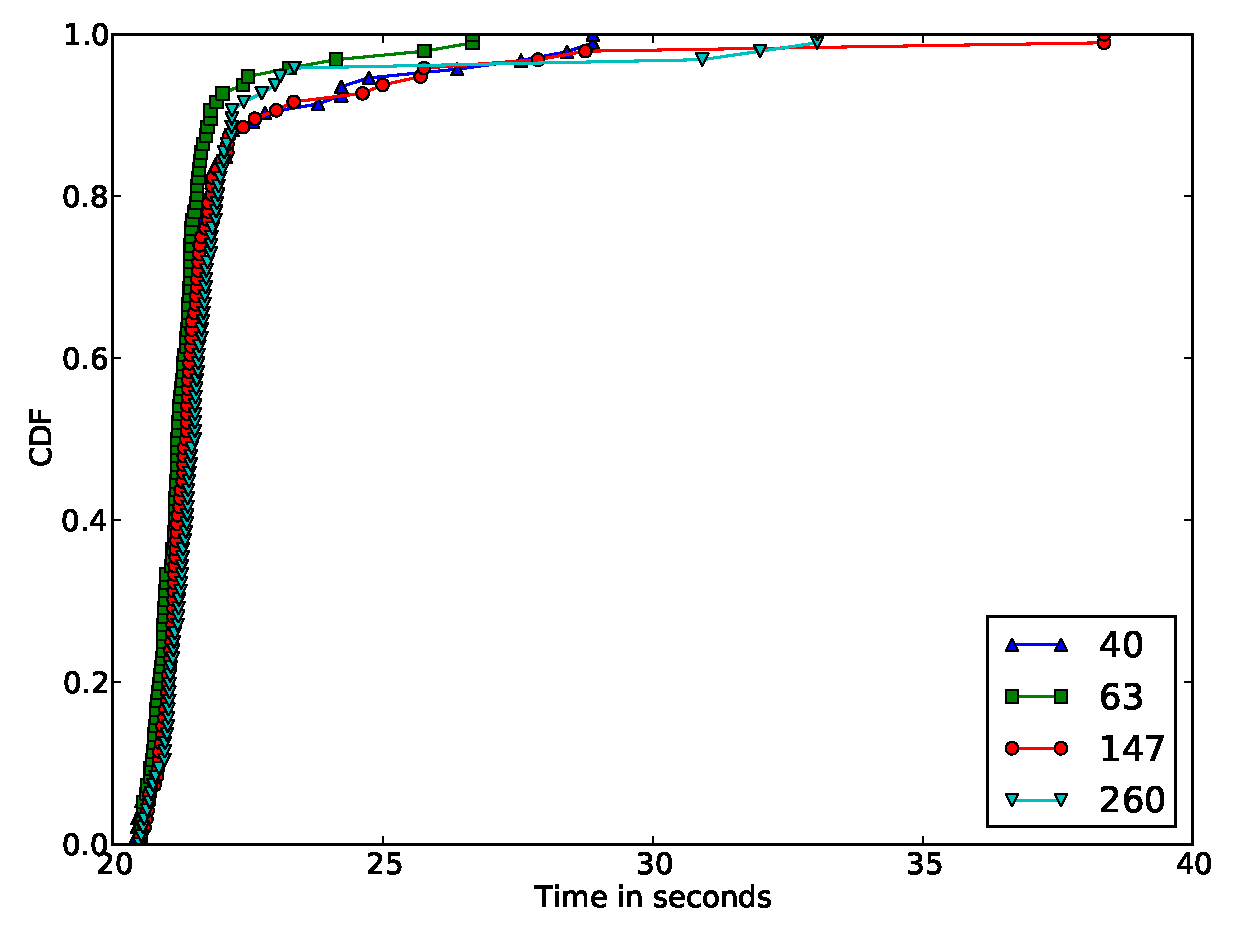
\includegraphics[width=2.5in]{figs/private.eps}
\caption{CDF of the time to bootstrap a private overlay node in a private
overlay of the size stated in the legend using a public overlay consisting of
600 nodes.  Using a 100 ms delay like the simulator results in 9.2 and 9.3
seconds for the analytical model for private network sizes of 68 and 147,
respectively.}
\label{fig:private_bootstrapping}
\end{figure}

Based upon the results presented in Figure~\ref{fig:private_bootstrapping}, the
bootstrapping time for the implementation performs better than the analytical
model, due to the simplicity of the analytical model and the small network
sizes.  It is of interest that while the simulator results tend to be in a well
defined range, the PlanetLab results have a few outliers with long bootstrap
times.  Some of the expected causes for this are churn in the system and state
machine timeouts in Brunet, though we have not considered this in this in much
depth in this work.

\subsection{Overhead of Pathing}

Much like the previous experiment, this verifies that the pathing technique has
negligible overheads for VPN usage.  To determine the overheads, two GroupVPNs
are deployed on resources on the same gigabit LAN.  To measure latency and
throughput, netperf experiments are run for 30 seconds, 5 times each on an
unutilized network switch.  Other specifications of the machine are ignored as
the system without pathing is used as the baseline.  The results,
Table~\ref{tab:pathing}, indicate that the use of pathing presents negligible
overhead for both throughput and latency, justifying the use of this approach
to transparently deal with NAT and firewall traversal.

\begin{table}[ht]
\centering
\begin{tabular}{|c||c|c|}
\hline & Latency (ms) & Throughput (Mbit/s) \\ \hline \hline
Standard & .303 & 225.27 \\ \hline
Pathing & .308 & 224.36 \\ \hline
\end{tabular}
\caption{Pathing overheads}
\label{tab:pathing}
\end{table}

\section{Security for the Overlay and the VPN}
\label{security}

Structured overlays are difficult to secure and a private overlay is not secure
if it provides no means to limit access to the system.  Malicious users can
pollute the DHT, send bogus messages, and even prevent the overlay from
functioning, rendering the VPN useless.  To address this in means that make
sense for VPNs and common users, we have employed a public key infrastructure
(PKI) to encrypt and authenticate both communication between peers as well as
communication across the overlay, called point-to-point (PtP) and end-to-end
(EtE) communication, respectively.

Use of a PKI motivates from the ability to authenticate without a third party,
ideal for P2P use, unlike a key distribution centers (KDC) used by other VPNs.
A PKI can use either pre-exchange public keys or a certificate authority (CA)
to sign public keys, i.e., certificates.  Thus peers can exchange keys and
certificates without requiring a third-party to be online.

The reasons for securing PtP and EtE are different.  Securing PtP communication
prevents unauthorized access to the overlay, as peers must authenticate with
each other for every link created.  Though once authenticated, a peer can
perform malicious acts and since the overlay allows for routing over it, the
peer can disguise the origination of the malicious acts.  By also employing EtE
security, the authenticity of messages transferred through an overlay can be
verified.  Though EtE security by itself, will not prevent unauthorized access
into the overlay.  By employing both PtP and EtE, overlays can be secured from
uninvited guests from the outside and can identify malicious users on the
inside.  Implementing both leads to important questions: what mechanisms can be
used to implement both and what are the effects of both on an overlay and to a
VPN on an overlay.

\subsection{Implementing Overlay Security}

There are various types of PtP links; for example, there are TCP and UDP
sockets, and relays across nodes and overlays.  EtE communication is
datagram-oriented in IPOP.  Traditional approaches of securing communication
such as IPsec are not convenient due to complexity, i.e., operating system
specific, portability constraints, and lack of common APIs.  Security protocols
that rely on reliable connections, such as SSL or TLS are undesirable as well
as they would require a userpace implementation of reliable streams (akin to
TCP).  As such, we have implemented an abstraction akin to a security filter as
presented in Figure~\ref{fig:security_filter}, which enables nearly transparent
use of security libraries and protocols.  To this date, we have implemented
both a DTLS~\cite{dtls} filter using the OpenSSL implementation of DTLS as well
as a protocol that reuses cryptographic libraries provided by .NET that behaves
similarly to IPsec.

A security filter has two components: the manager, and individual sessions or
filters.  While the individual sessions could act as filters by themselves, by
combining with a manager, they can be configured for a common purpose and
security credentials.  This approach enables the use of security to be
transparent to the other components of the system as the manager handles
session establishment, garbage collection of expired sessions, and revocation
of peers.

\begin{figure}[ht]
\centering
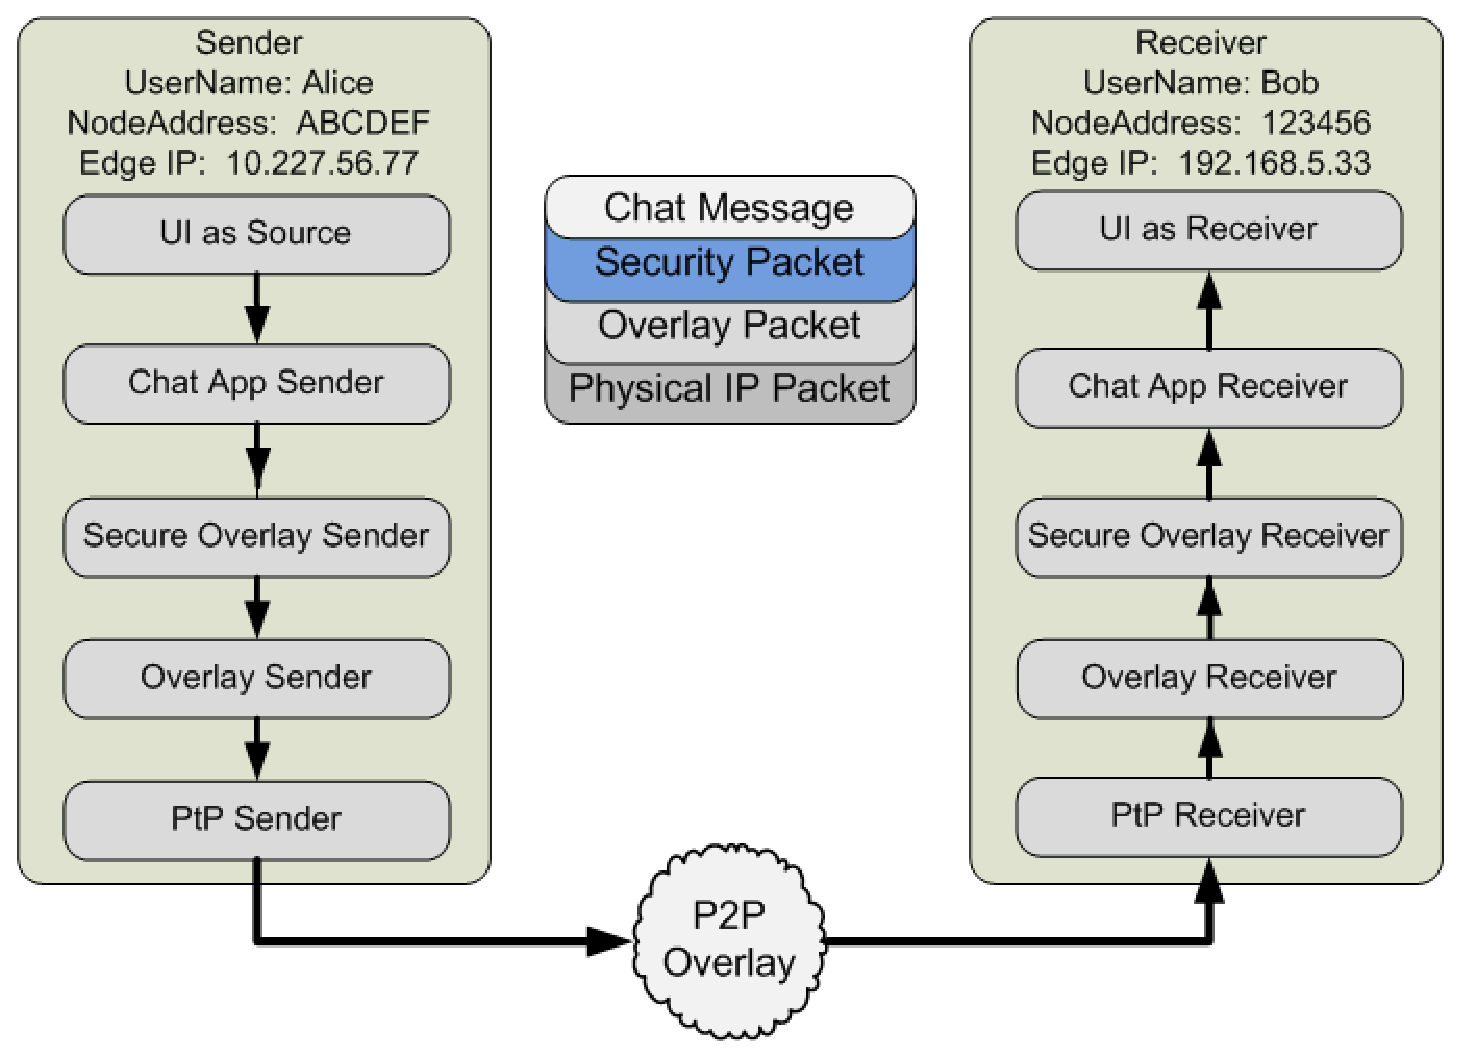
\includegraphics[width=3in]{figs/secure_sender_stack_generic.png.eps}
\caption{An example of the abstraction of senders and receivers using a EtE 
secured chat application.  Each receiver and sender use the same abstracted
model and thus the chat application requires only high-level changes, such
as verifying the certificate used is Alice's and Bob's, to support security.}
\label{fig:security_filter}
\end{figure}

Certificate embed identity of the owner, thus a signed certificate states that
the signer trusts that the identity is accurate.  In network systems, the
certificate uses the domain name to uniquely identify and limit the use of a
certificate.  When a CA signs the certificate, by including the domain name, it
ensures that users can trust that a certificate is valid, while used to secure
traffic to that domain.  Communication with another domain using the same
certificate will raise a flag and will result in the user not trusting the
certificate.  In environments with NATs, dynamic IP addresses, or portable
devices, typical of P2P systems, assigning a certificate to a domain name will
be a hassle as it constrains mobility and the type of users in the system.
Furthermore, most users are unaware of their IP address and changes to it.
Instead, a certificate is signed against the user's P2P address and unique user
name as delegated by the CA.  The purpose of the former is for efficiency of
revocation as discussed in Section~\ref{revocation}.  During the formation of
PtP links or while parsing EtE messages, the two nodes discover each other's
P2P addresses.  If the addresses do not match the address on the verified
certificate, the communication need not proceed further.  

Prior to trusting the security filter, the core software or the security filter
must ensure that the P2P address of the remote entity matches that of the
certificate.  In our system, we did this by means of a callback, which presents
the underlying sending mechanism, EtE or PtP, and the overlay address stored in
the certificate.  The receiver of the callback can attempt to cast it into
known objects. If successful, it will compare the overlay address with the
sender type.  If unsuccessful, it ignores the request.  If any callbacks return
that the sender does not match the identifier, the session is immediately
closed.  Thus the security filter need not understand the sending mechanism and
the sending mechanism need not understand the security filter.

The last consideration comes in the case of EtE communication that provides an
abstraction layer.  For example, in the case of VPNs, where a P2P packet
contains an IP packet and thus a P2P address maps to a VPN IP address, a
malicious peer may establish a trusted link, but then hijack another users IP
session.  As such, the application must verify that the IP address in the IP
packet matches the P2P address of the sender of the P2P packet.  In general, an
application address should be matched against a P2P address, consider chat
programs, for example.

\subsection{Overheads of Overlay Security}

When applying an additional layer to a P2P system, there are overheads in terms
of time to connect with the overlay.  Other less obvious effects will be
throughput, latency, and processing overheads, assuming that the P2P system
will be used over a wide area network, where the latency and throughput
limitations between two points will make the overhead of security negligible.
Though bootstrapping will be affected due to additional round trip messages
used for forming secure connections.

\begin{figure}[ht]
\centering
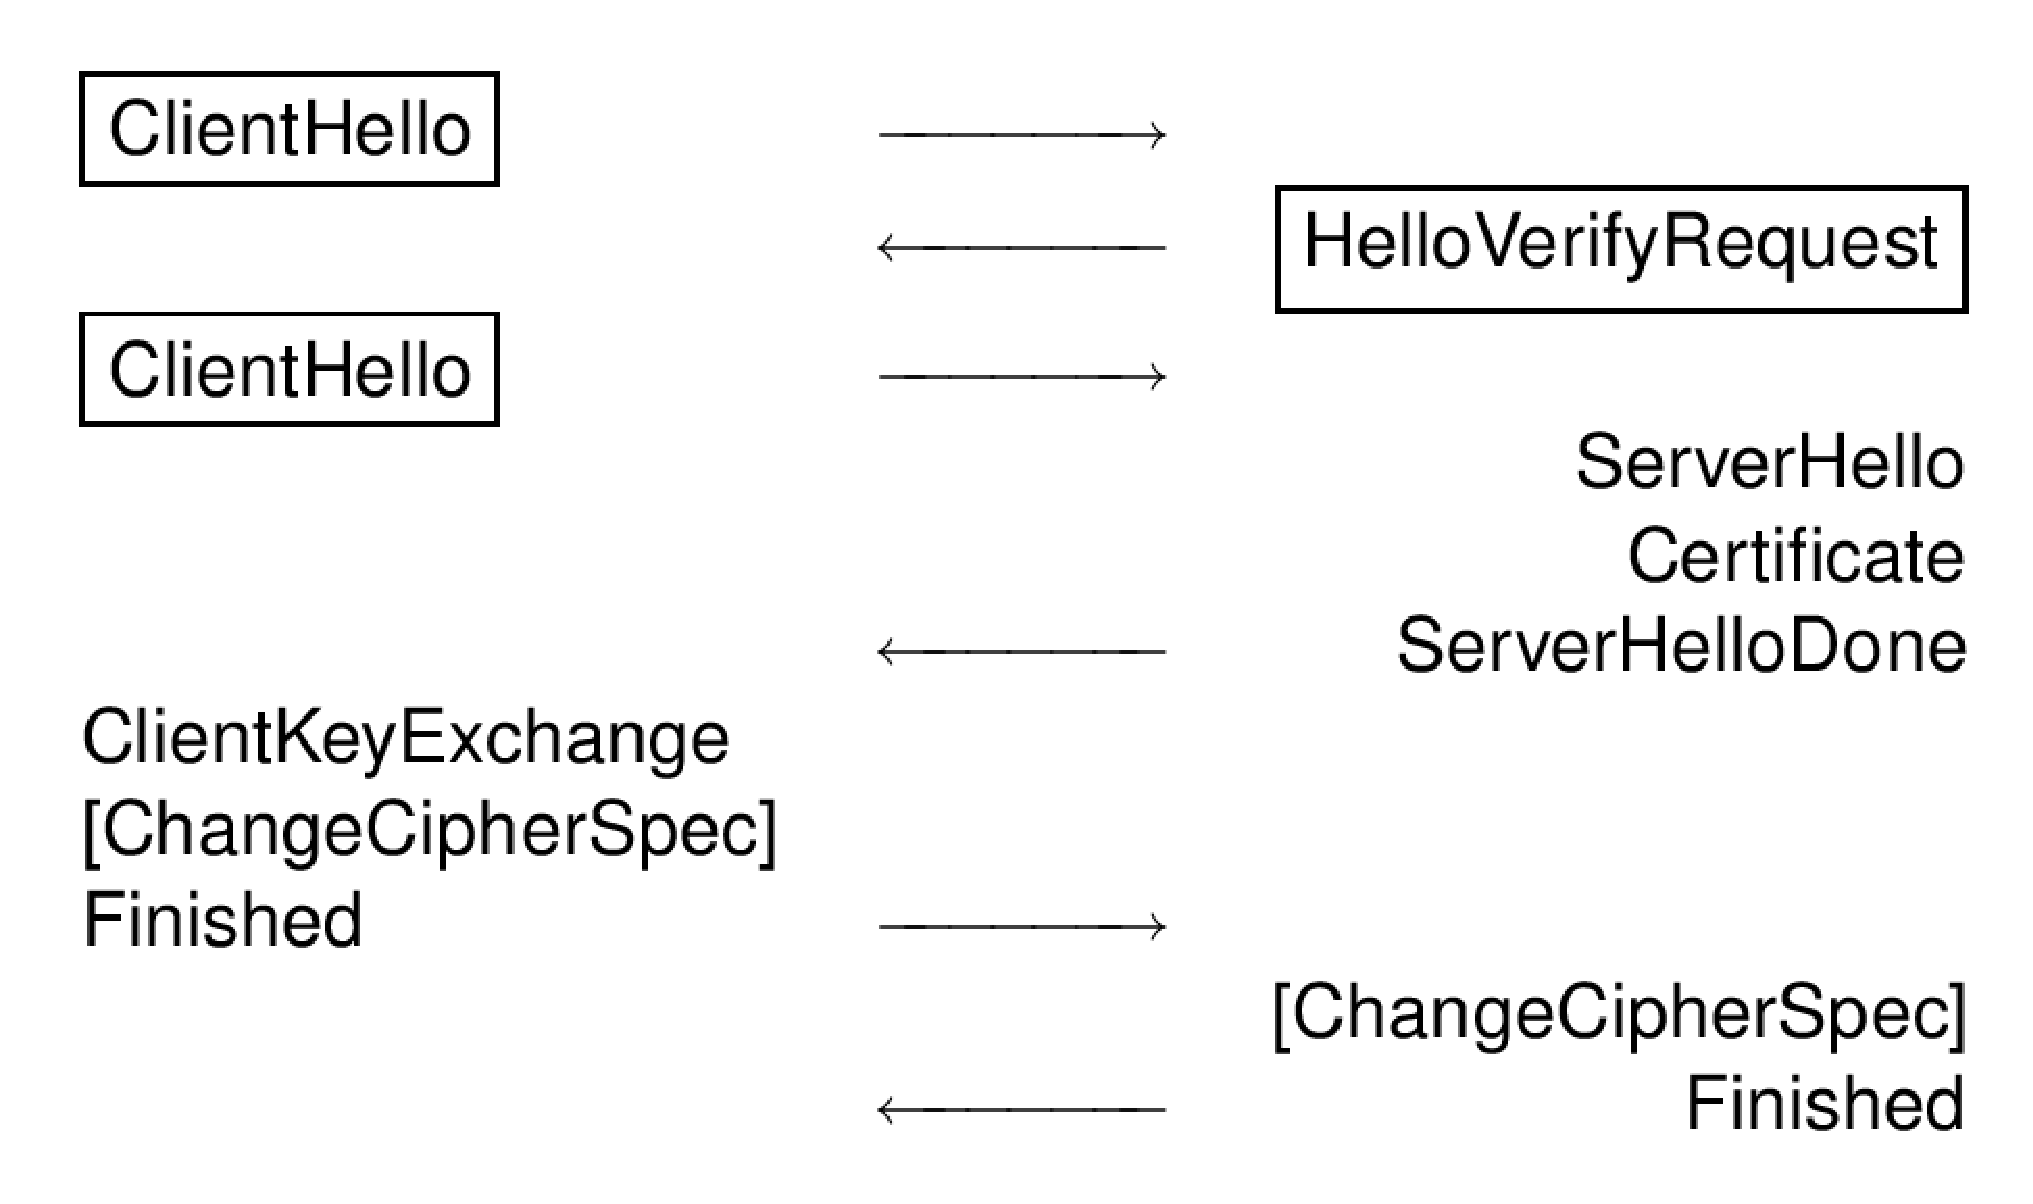
\includegraphics[width=2.5in]{figs/dtls.eps}
\caption{DTLS handshake}
\label{fig:dtls}
\end{figure}

The DTLS handshake as presented in Figure~\ref{fig:dtls}, which consists of 6
messages or 3 round trips.  PtP security may very well have an effect on the
duration of overlay bootstrapping.  There even exists a possibility that with
more messages during bootstrap, the probability one drops is higher, which
could, in turn, also have an effect, though possibly negligible, on time to
connect.  To evaluate these concerns, we have employed both simulation and real
system experiments.

The following experiments use both simulation and PlanetLab deployment to
evaluate time to connect a new node to an existing resource.  Then another
experiment is performed to evaluate how long it takes to bootstrap various
sized overlays if all nodes join at the same time.  This experiment is only
feasible via simulation as attempting to reproduce in a real system is
extremely difficult due to how quickly the operations complete.

\subsubsection{Adding a Single Node}

This experiment determines how long it takes a single node to join an existing
overlay with and without DTLS security.  The experiment is performed using both
simulation and PlanetLab.  After deploying a set of nodes without security and
with security on PlanetLab, the network is crawled to determine the size of the
network.  In both cases, the overlay maintained an average size of around 600
nodes.  At which point, we connected a node 1,000, each time using a new,
randomly generated P2P address, thus connecting to a different point in the
overlay.  The experiment concludes as soon as the node has connected to the
peers in the P2P overlay immediately before and after it in the P2P address
space.  In the simulation, a new overlay is created and afterward a new node
joins, this is repeated 100 times.  The cumulative distribution functions
obtained from the different experiments are presented in
Figure~\ref{fig:add_one}.

\begin{figure}[ht]
\centering
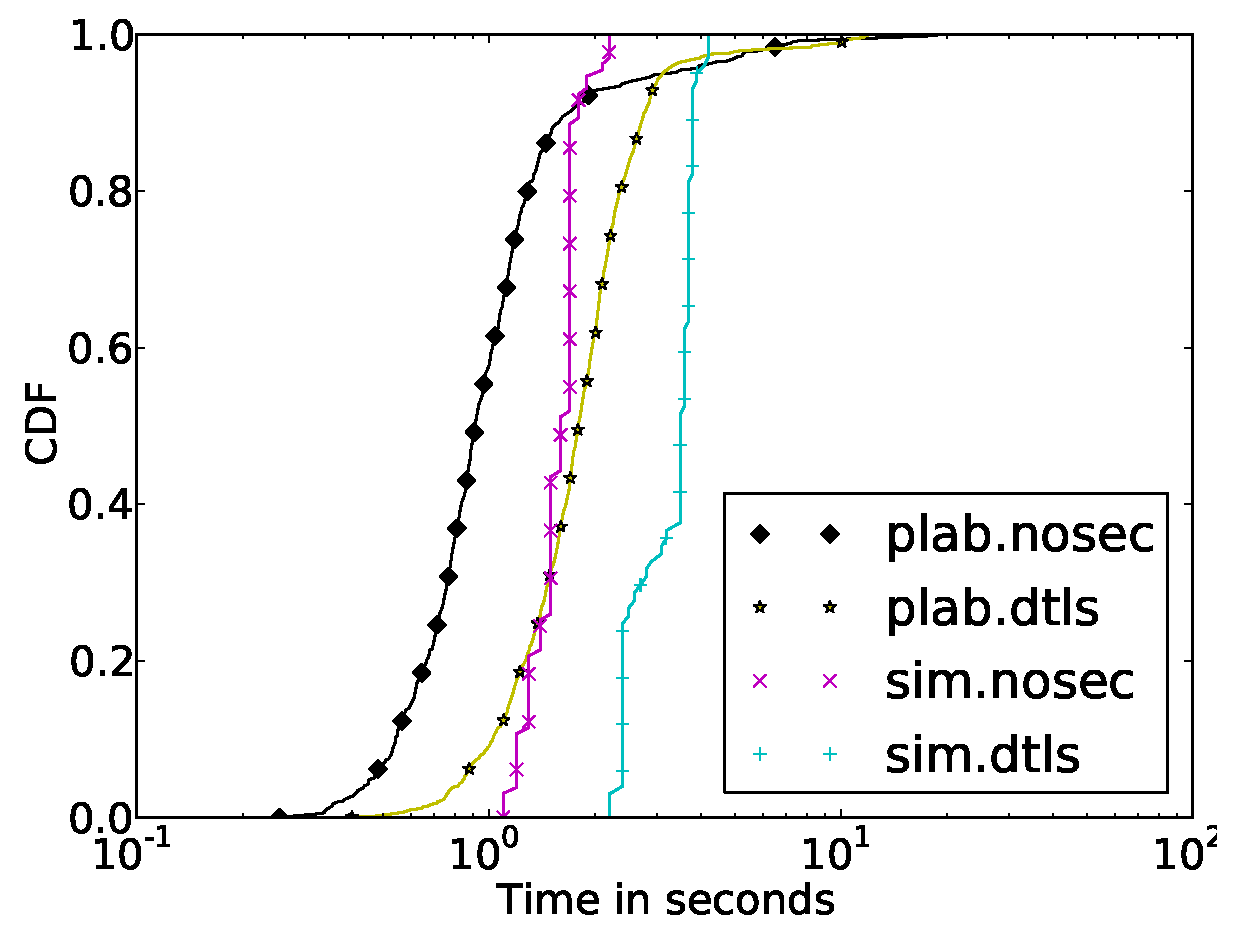
\includegraphics[width=2.5in]{figs/addone.eps}
\caption{Time in seconds for a single node to join a secure (dtls) and insecure
(nosec) structured overlay, using both PlanetLab (plab) and the Simulator
(sim).}
\label{fig:add_one}
\end{figure}

\subsubsection{Bootstrapping an Overlay}

The purpose of this experiment is to determine how quickly an overlay using
DTLS can bootstrap in comparison to one that does not given that there are no
existing participants.  Nodes in this evaluation are randomly given information
about 5 different nodes in the overlay and then all attempt to connect with
each other at the same time.  The evaluation completes after the entire overlay
has all nodes connected and in their proper position.  For each network size,
the test is performed 100 times and the average result is presented in
Figure~\ref{fig:bootstrap_eval}.

\begin{figure}[ht]
\centering
\includegraphics[width=2.5in]{figs/bootstrap.eps}
\caption{Time in seconds for a secure (dtls) and insecure (nosec) structured
overlay to bootstrap, given that all nodes bootstrap simulataneously.}
\label{fig:bootstrap_eval}
\end{figure}

\subsection{Discussion}

Both evaluations show that the overhead in using security is practically
negligible, when an overlay is small.  In the case of adding a single node, it
is clear that the simulation and deployment results agree, as the difference
between bootstrapping into an overlay with and without security remains nearly
the same.  Clearly this motivates the use of security if time to connect is the
most pressing question.

The time to bootstrap a secure overlay was not significantly more than that of
an insecure overlay.  What we realized is that complex connection handshaking,
as implemented in Brunet, seems to dominate connection establishment time.  For
example, in Brunet, two peers must communicate via the overlay prior to forming
a connection, and the system differentiates between bootstrapping connections
and overlay connections.  Thus even though a peer may have a bootstrapping
connection, it will need to go through the entire process to form an overlay
connection with a peer.  While this may lead to inefficiencies, this
simplification keeps the software more maintainable and easier to understand.

\section{Handling User Revocation}
\label{revocation}

Unlike decentralized systems that use shared secrets, in which the creator of
the overlay becomes powerless to control malicious users, PKIs enable their
creators to effectively remove malicious users.  Typical PKIs either use a
certificate revocation list (CRL) or online certificate verification protocols
such as Online Certificate Status Protocol (OCSP).  These approaches are
orthogonal to decentralized systems as they require a dedicated service
provider.  If the service provider is offline, an application can only rely on
historical information to make a decision on whether or not to trust a link.
In a decentralized system, these features can be enhanced so not to rely on a
single provider.  In this section, we present two mechanisms of doing so:
storing revocations in the DHT and performing overlay broadcast based
revocations.

\subsection{DHT Revocation}

A DHT can be used to provide revocation similar to that of OCSP or CRLs.
Revocations, a hash of the certificate and a time stamp signed by the CA, are
stored  are stored in the DHT at the key formed by the hashing of the
certificate.  In doing so, revocations will be uniformly distributed across the
overlay, not relying on any single entity.

The problem with the DHT approach is that it does not provide an event
notification for members currently communicating with the peer.  While peers
could continue to poll the DHT to determine a revocation, doing so is
inefficient.  Furthermore, a malicious peer, who has a valid but revoked
certificate could force every member in the overlay to query the DHT,
negatively affecting the DHT nodes storing the revocation.

\subsection{Broadcast Revocation}

Broadcast revocation can be used to address the deficiencies of DHT revocation.
As a topic of previous research works~\cite{broadcast, chord_broadcast},
structured overlays can be used without additional state to perform efficient
broadcasts from any point in the overlay to the entire overlay.  The form of
broadcast can be used to perform to notify the entire overlay immediately about
a new revocation.  In these papers, analysis and simulations have shown that
the approach can be completed in $O(\log^2 n)$ time.

\begin{figure}[ht]
\centering
\includegraphics[width=2.5in]{figs/tree.eps}
\caption{Broadcast performing a complete overlay broadcast}
\label{fig:tree}
\end{figure}

Our modified algorithm as illustrated in Figure~\ref{fig:tree} utilizes the
organization of a structured system with a circular address space that requires
peers be connected to those whose node addresses are the closest to their own,
features typical of one-dimensional structured overlays including
Chord~\cite{chord}, Pastry~\cite{pastry}, and Symphony.  Using such an
organization, it is possible to do perform a broadcast with no additional
state.  To perform a broadcast, each node performs the following recursive
algorithm:

\begin{algorithmic}
\STATE {\bf BROADCAST(start, end, message)}:
  \STATE RECEIVE(message)
  \FOR{$i$ in length(connections)}
    \STATE n\_start $\gets$ ADDRESS(connections$[i]$)
    \IF {n\_start $\not\in$ $[$start, end$)$}
      \STATE continue
    \ENDIF
    \STATE n\_end $\gets$ ADDRESS(connections$[i+1]$)
    \IF {n\_end $\not\in$ $[$start, end$)$}
      \STATE n\_end $\gets$ end
    \ENDIF
    \STATE msg $\gets$ (BROADCAST, n\_start, n\_end, message)
    \STATE SEND(connections$[i]$, msg)
  \ENDFOR
\end{algorithmic}
with ``connections'' as a circular list of connections in non-decreasing order
from the perspective of the node performing the current recursive, broadcast
step.

In this algorithm, the broadcast initiator uses its own address as the start
and end, thus the broadcast will span the entire overlay after completing
recursive calls at each connected node.  A recursive end, ``n\_end'', must be
inside the region between ``start'' and ``end'', thus if the connection
following the current sending connection, ``connections$[i+1]$'', is not in
that region, it will only broadcast up to ``end'' and not the address specified
by that connection.  Finally, nodes, who have a connection to the malicious
peer, will end the connection prior to accidentally forwarding the message to
the peer by receiving and acting upon the revocation prior to forwarding the
message.  To summarize, the overlay is recursively partitioned amongst the
nodes at each hop in the broadcast.  By doing so, all nodes receive the
broadcast without receiving duplicate broadcast messages.

\subsection{Evaluation of Broadcast}

We performed an evaluation on the broadcast using the simulation to determine
how quickly peers in the overlay would receive the message.  The tested network
sizes ranged from 2 to 256 in powers of 2.  The tests were evaluations were
performed 100 times for each network size.  The CDF of hops for each node are
presented in Figure~\ref{fig:broadcast}.  The results make it quite clear that
the broadcast can efficiently distribute a revocation much more quickly than
$\log(N)$ time.

\begin{figure}[ht]
\centering
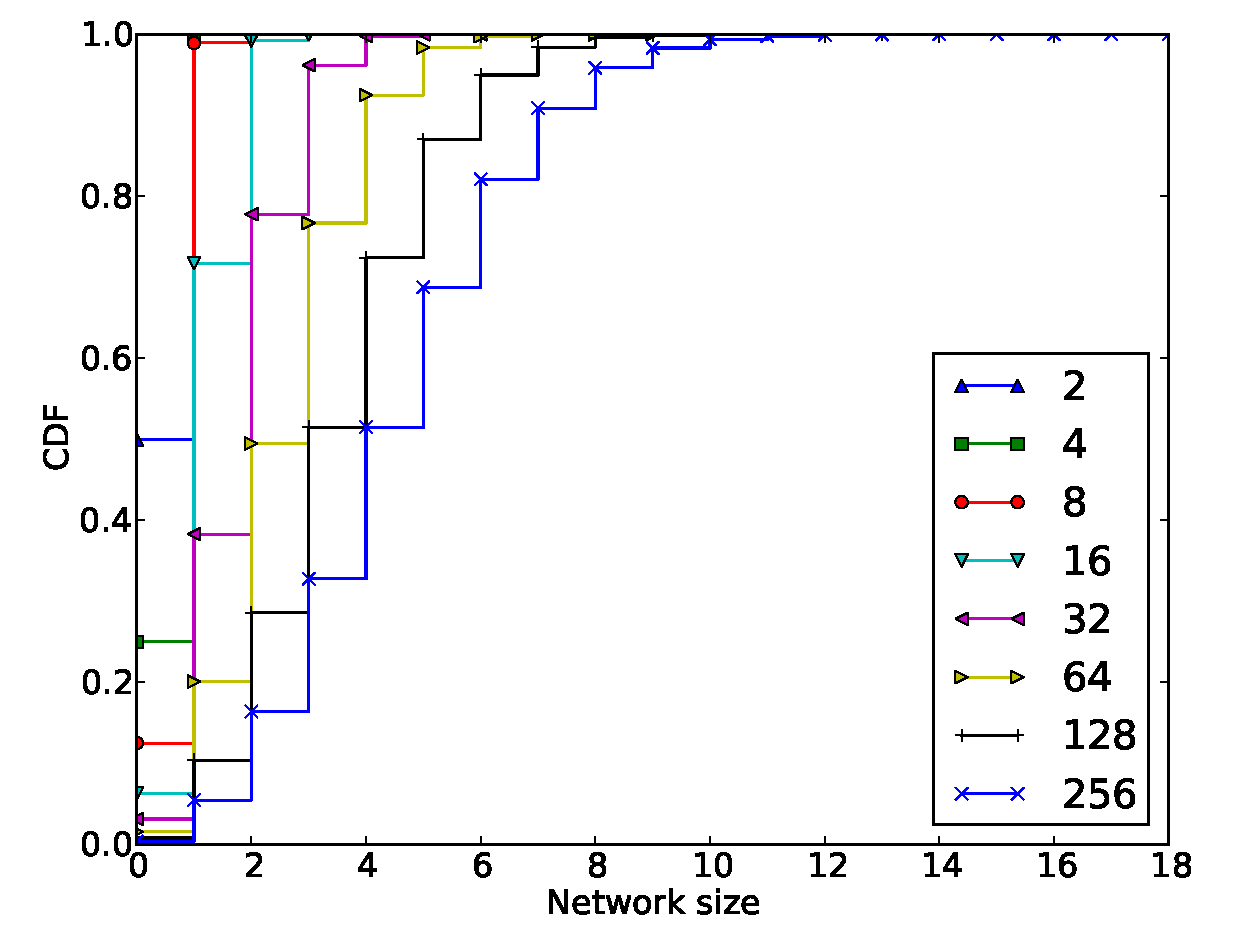
\includegraphics[width=2.5in]{figs/broadcast.eps}
\caption{Overlay broadcast time CDF.}
\label{fig:broadcast}
\end{figure}

\begin{figure*}[ht]
\centering
\includegraphics[width=2.5in,angle=-90]{figs/groupvpn.ps}
\caption{Process in bootstrapping a new GroupVPN instance.}
\label{fig:groupvpn}
\end{figure*}

\subsection{Discussion}

In contrast to the DHT solution, broadcast revocation occur only once and leave
no state behind.  Thus the broadcast is not a complete solution, as new peers
connected to the overlay or those who missed the broadcast message will be
unaware of a revocation.  Furthermore, if an overlay is shared by many VPNs, it
may prevent overlay broadcasting or itself may be inefficient.

The DHT solution by itself may also not sufficient as revocations may be lost
over time as the entries must have their leases renewed in the DHT.  To address
this condition, each peer maintains a local CRL and the owner of the overlay
can occasionally send updates to the CRL through an out of band medium, such as
e-mail.  A better long term solution may be the use of a gossip protocols so
that peers can share their lists with each other during bootstrapping phases.

A key assumption in using these is that a Sybil~\cite{sybil}, or collusion
attack, is difficult in the secured overlay.	 If a Sybil attack is successful,
both a DHT and broadcast revocation may be unsuccessful, though peers could fix
this problem by obtaining the CRL out of band.  In addition, previous
work~\cite{secure_routing} has described decentralized techniques to limit the
probability of such attacks from occurring.  In our approach, the use of
central authority to review certificate requests can be used to limit a single
user from obtaining too many certificates as well as ensuring uniform
distribution of that user's P2P addresses, further hampering the likelihood of
a Sybil attack.  The ability to automate this is left as future work.

One way to mitigate sybil attacks using the broadcast approach is to bundle
colluding offenders into a single revocation message.  That would prevent those
from colluding together to prevent each other's revocations.  Furthermore,
while not emphasized above, revocation in our system revokes by user name and
not individual certificates.  Combined these two components limit sybil attacks
against broadcast.

\section{Managing and Configuring the VPN}
\label{groupvpn}

While the PKI model applies to P2P overlays, actual deployment and maintenance
of security credentials can be too complex to manage, particularly for
non-experts.  Most PKI-enabled systems require the use of command-line
utilities and lack methods for assisting in the deployment of certificates and
policing users.  Our solution to facilitate use of PKIs for non-experts is a
partially-automated PKI reliant on a group-based Web interface distributable in
forms of Joomla add-ons as well as a virtual machine appliance.  In this
environment, groups can share a common Web site, while each group has their own
unique CA.  Although this does not preclude other methods of CA interaction,
experience has shown that it provides a model that is satisfactory for many use
cases.

Group-based Web 2.0 sites enable low overhead configuration of collaborative
environments.  The roles in a group environment can be divided into
administrators and users.  Users have the ability to join and create groups;
whereas administrators define network parameters, can accept or deny join
requests, remove users, and promote other users to administrators.  By applying
this to a VPN, the group environment provides a simple to use wrapper around
PKI, where the administrators of the group act as the CA and the members have
the ability to obtain signed certificates.  

Elaborating further, when a user joins a group, the administrator can enable
automatic signing of certificates or require prior review; and when peers have
overstayed their welcome, an administrator can revoke their certificate by
removing them from the group.  Revocations are handled as described in
Section~\ref{revocation}.  In the context of GroupVPN systems, a user
revocation list as opposed to a CRL simplifies revocation, since users and not
individual certificates will be revoked.

Registered users who create groups become administrators of their own groups.
When a user has been accepted into a group by its administrator, they are able
to download VPN configuration data from the Web site.  Configuration data is
loaded by the GroupVPN during its configuration process to specify IP address
range, namespace, and security options.  The configuration data also stores a
shared secret, which uniquely identifies the user, enabling the Web site to
automatically sign the certificate (or enqueue it form manual signing,
depending on the group's policy).  Certificate requests consist of sending a
public key and a shared secret over an HTTPS connection to the web server.
Upon receiving the signed certificate, peers are able to join the private
overlay and GroupVPN, enabling secure communication amongst the VPN peers.  The
entire bootstrapping process, including address resolution and communication
with a peer, is illustrated in Figure~\ref{fig:groupvpn}.

There are many ways of implementing and hosting the Web site.  For example,
Google offers free hosting of Python web applications through Google Apps, an
option available if the user owns a domain.  Alternatively, the user could host
the group site on a public virtual network. In this case, peers interacting
with the GroupVPN would need to connect with the public virtual network in
order to create an account, get the configuration data, and retrieve a signed
certificate, at which point they could disconnect from it.  This does not
preclude the use of other social mediums nor a central site dedicated to the
formation of many GroupVPNs.  Many GroupVPNs can share a single site, so long
as the group members trust the site to host the CA private key.

\section{Related Work}
\label{related_work}

\subsection{VPNs}

Hamachi~\cite{hamachi} is a centralized P2P VPN provider using the web site for
authentication, peer discovery, and connection establishment.  While the
Hamachi protocol claims to support various types of
security~\cite{hamachi_security}, the implementation appears to only support
the key distribution center (KDC) requiring that all peers establish trusted
relationship through the central website.  The Hamachi approach makes it easy
for users to deploy their own services, but places limitations on network size,
uses a proprietary security stack, and does not allow independent VPN
deployments.  In contrast, our approach presents a completely decoupled
environment allowing peers to start using our shared system to bootstrap
private overlays and migrate away without cost if need be.  Furthermore our
approach relies only on a central server to obtain the certificate otherwise,
it is decentralized.  In Hamachi, if the central server goes offline, no new
peers can join the VPN.

Campagnol VPN~\cite{campagnol} provides similar features to Hamachi: a P2P VPN
that relies on a central server for rendezvous or discovery of peers.  The key
differences between Hamachi and Campagnol is that Campagnol is free and does
not provide a service; users msut deploy their own rendezvous service.  The
authors of Campagnol also state that the current approach limits the total
number of peers sharing a VPN to 100 so not to overload the rendezvous service.
The current implementation does not support a set of rendezvous nodes, though
doing so would make the approach much more like ours.  In addition, the system
relies on traditional distribution of a CRL to handle revocation.

Tinc~\cite{tinc} is a decentralized VPN requiring users to manually organize an
overlay with support for finding optimal paths.  In comparison to our approach,
Tinc does not automatically handle churn in the VPN.  If a node connecting two
separate pieces of the VPN overlay goes offline, the VPN will be partitioned
until a user manually creates a link connecting the pieces.  Furthermore, Tinc
does not form direct connections for improved latency and throughput reasons,
thus members acting as routes in the overlay incur the price of acting as
packet forwarders.

The last VPN, we discuss is the most similar like ours, its called
N2N~\cite{n2n}.  N2N uses unstructured p2p techniques to form an Ethernet based
VPN.  While their approach, like ours, has built-in NAT traversal, it requires
that users deploy their own bootstrap and limits security to a single
pre-shared key for the entire VPN, thus users cannot be revoked.  Since N2N
provides Ethernet, users must provide their own mechanism for IP address
allocation, while discovery utilizes overlay broadcasting.  Thus there are
concerns that as systems get larger, N2N may not be very efficient.

\subsection{P2P Systems}

BitTorrent~\cite{bittorrent_security}, a P2P data sharing service,  supports
stream encryption between peers sharing files.  The purpose of BitTorrent
security is to obfuscate packets to prevent traffic shaping due to packet
sniffing. Thus BitTorrent security uses a weak stream cipher, RC4, and lacks
peer authentication as symmetric keys are exchanged through an unauthenticated
Diffie-Hellman process.

Skype~\cite{skype} provides decentralized audio and video communication to over
a million concurrent users.  While Skype does not provide documentation
detailing the security of its system, researchers~\cite{skype_auth,
skype_overview} have discovered that Skype supports both EtE and PtP security.
Though similar to Hamachi, Skype uses a KDC and does not let users setup their
own systems.

As of December 2009, the FreePastry group released an SSL enabled
FreePastry~\cite{pastry}.  Though relatively little is published regarding
their security implementation, the use of SSL prevents its application for use
in the overlay and for overlay links that do not use TCP, such as relays and
UDP.  Thus their approach is limited to securing environments that are not
behind NATs and firewalls that would prevent direct TCP links from forming
between peers.

\section{Conclusions}
\label{conclusions}

This paper overviews the architecture implementation of GroupVPN, a system that
is the first to demonstrate the practical feasibility of using structured
overlays as a basis for easy-to-use, group-oriented, P2P VPNs.  Explicitly, we
have taken common structured overlays and explored organization, public
overlays for connectivity, and private overlays for security and then described
our GroupVPN which binds them the components together to create collaborative
environments for configuration and management of VPNs.  This paper extends upon
the IPOP virtual network to support user-friendly approaches for users to
create and manage their own virtual private networks.  To accomplish this, each
IPOP system bootstraps into its own unique, secure P2P overlay.  This approach
not only enables secure communications in IPOP deployments but also enables for
more efficient overlay multicast and broadcast.

The use of service overlays significantly improves performance and maintenance.
Peers can easily control membership in the overlay and it presents unique
opportunities for decentralized revocation.  A DHT approach allows results to
be stored on the overlay instead of using centralized CRLs and broadcast to
immediately notify active participants of a revocation.  Ongoing work include
investigating slow bootstrap times and determining security concerns of the
decentralized revocation techniques.  Furthermore, we plan on investigating the
use of overlay broadcasting for IP broadcasting and multicasting, though the
current approach places an unfair burden on the first few hops of a broadcast.

Without the functionality of GroupVPN, projects like the Grid Appliances and
its flagship application, Archer~\cite{archer}, would be impractical.  Archer
consists of over 500 resources from 5 different universities, including
University of Florida, Florida State University, Northeastern University,
University of Minnesota, and University of Texas.  In the past year, since
Archer came online, over 100 unique users have contributed and taken advantage
of the voluntary computing cycles.  The use of existing decentralized VPNs in
Archer and the Grid Appliance would be severely limiting.  In the case of N2N,
at least one peer would have to maintain the bootstrap service and address
allocations for the VPN.  Tinc would require users to manually configure their
networking overlays.  While Compagnol and Hamachi require the use of well known
centralized peers.  

The GroupVPN has been used as the virtual network for the Grid Appliance,
enabling the creation of decentralized, collaborative environments for
computing grids.  Recently, grids at La Jolla Institute for Allergy and
Immunology and two in Eastern Europe went live using GroupVPN without receiving
any technical support from us.  Researchers at Clemson University and Purdue
have opted for this approach over centralized VPNs as the basis of their future
distributed compute clusters and have actively tested networks of over 700
nodes.

\section*{Acknowledgments}
 
We thank the anonymous reviewers as well as Pierre St. Juste for their useful
comments and feedback.  This research is sponsored by the National Science
Foundation under grants IIP-0758596 and CNS/CRI collaborative awards 0751112,
0750847, 0750851, 0750852, 0750860, 0750868, 0750884, and 0751091. Any
opinions, findings and conclusions or recommendations expressed in this
material are those of the authors and do not necessarily reflect the views of
the NSF.

\small{
\bibliographystyle{IEEEtran}
\bibliography{GroupVPN}
}

\end{document}
